\documentclass[border=0.25in]{standalone}
\usepackage{tikz}
\usepackage{xcolor}
\usepackage{array}
\usetikzlibrary{shapes.misc, patterns}

\begin{document}
%%%%%%%%%%%%%%%%%%%%%%%%%%%%%%%%%%%%%%%%%%%%%%%%%%
%%%%%%%%%%%%%%%%%%%%%%%%%%%%%%%%%%%%%%%%%%%%%%%%%%
\begin{tabular}{c c}

% Expt EV
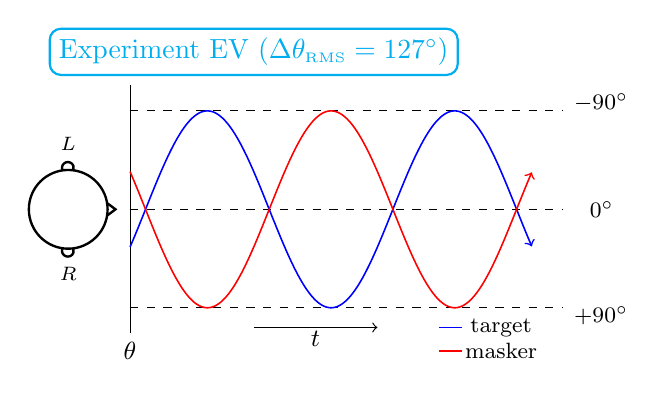
\begin{tikzpicture}
  % Title
  \node[thick, draw=cyan, text=cyan, rounded corners, opacity=1] at (3*pi/4, 2) {Experiment EV ($\Delta \theta_{\textrm{\tiny RMS}} = 127^{\circ}$)};
  
  % Legend
  \draw[line width=0.2mm, blue] (3*pi/2, -1.5) -- (3*pi/2 + 3*pi/32, -1.5);
  \node at (3*pi/2 + 8*pi/32, -1.5) {\footnotesize target};
  \draw[line width=0.2mm,  red] (3*pi/2, -1.8) -- (3*pi/2 + 3*pi/32, -1.8);
  \node at (3*pi/2 + 8*pi/32, -1.8) {\footnotesize masker};
  
  % y axis
  \draw[line width=0.125mm, black] (pi/4, -1.575) -- (pi/4, 1.575);
  \node at (pi/4, -1.8) {\small $\theta$};
  
  % Dashed degree guide lines
  \draw[line width=0.125mm, black, dashed] (pi/4,  1.25) -- (2*pi,  1.25);
  \draw[line width=0.125mm, black, dashed] (pi/4,  0.)   -- (2*pi,  0.  );
  \draw[line width=0.125mm, black, dashed] (pi/4, -1.25) -- (2*pi, -1.25);
  
  % Degree guides
  \node[align=right, text width=0.5cm] at (2*pi + pi/8,  1.35)
    {\footnotesize $-90^{\circ}$};
  \node[align=right, text width=0.5cm] at (2*pi + pi/8,  0.)
    {\footnotesize $0^{\circ}$};
  \node[align=right, text width=0.5cm] at (2*pi + pi/8, -1.35)
    {\footnotesize $+90^{\circ}$};
  
  % Arrow of time
  \draw[help lines, ->, line width=0.15mm, black] (3*pi/4, -1.5) -- (5*pi/4, -1.5);
  \node at (pi, -1.65) {\small $t$};
  
  % Sinusoids
  \draw[help lines, ->, line width=0.2mm, blue, domain=pi/4:2*pi - pi/8, samples=1000]
        plot(\x, {-1.25*sin((2*\x + 3*pi/8) r)});
  \draw[help lines, ->, line width=0.2mm,  red, domain=pi/4:2*pi - pi/8, samples=1000]
        plot(\x, { 1.25*sin((2*\x + 3*pi/8) r)});
  
  % Head
  \node at (0, 0.825) {\scriptsize $L$};
  \draw[line width=0.3mm] (0, 0) circle (0.5cm); % head
  \draw[line width=0.3mm] (0 - 0.075,  0.5) arc ( 200:-20:0.075); % R ear
  \draw[line width=0.3mm]
         (0 + 0.5,  0.075) --
         (0 + 0.6,  0.   ) --
         (0 + 0.5, -0.075); % nose
  \draw[line width=0.3mm] (0 - 0.075, -0.5) arc (-200: 20:0.075); % L ear
  \node at (0, -0.825) {\scriptsize $R$};
\end{tikzpicture}
&



%%% Expt EV stim conditions
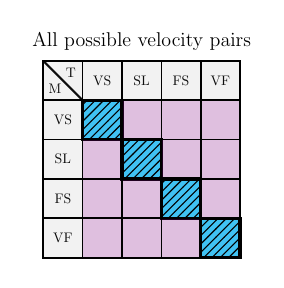
\begin{tikzpicture}[scale=0.5, every node/.style={transform shape}]
  \node at (2.5, 5.5) {\Large All possible velocity pairs};

  % Target/Masker
  \node at (0.7, 4.7) {T};
  \node at (0.3, 4.3) {M};
  \draw[thick] (0, 5) -- (1, 4);
  
  % Row labels
  \node at (1.5, 4.5) {VS};
  \node at (2.5, 4.5) {SL};
  \node at (3.5, 4.5) {FS};
  \node at (4.5, 4.5) {VF};
  % Column labels
  \node at (0.5, 3.5) {VS};
  \node at (0.5, 2.5) {SL};
  \node at (0.5, 1.5) {FS};
  \node at (0.5, 0.5) {VF};
  
  % Row 1 (top)
  \draw[semithick, draw=black, fill=gray, fill opacity=0.1]
     (0, 4) -- (0, 5) -- (1, 5) -- (1, 4) -- cycle;
  \draw[semithick, draw=black, fill=gray, fill opacity=0.1]
     (1, 4) -- (1, 5) -- (2, 5) -- (2, 4) -- cycle;
  \draw[semithick, draw=black, fill=gray, fill opacity=0.1]
     (2, 4) -- (2, 5) -- (3, 5) -- (3, 4) -- cycle;
  \draw[semithick, draw=black, fill=gray, fill opacity=0.1]
     (3, 4) -- (3, 5) -- (4, 5) -- (4, 4) -- cycle;
  \draw[semithick, draw=black, fill=gray, fill opacity=0.1]
     (4, 4) -- (4, 5) -- (5, 5) -- (5, 4) -- cycle;
  % Row 2
  \draw[semithick, draw=black, fill=gray, fill opacity=0.1]
     (0, 3) -- (0, 4) -- (1, 4) -- (1, 3) -- cycle;
  \draw[very thick, draw=black, fill=cyan, fill opacity=0.75]
     (1, 3) -- (1, 4) -- (2, 4) -- (2, 3) -- cycle;
  \draw[semithick, draw=black, pattern=north east lines]
     (1, 3) -- (1, 4) -- (2, 4) -- (2, 3) -- cycle;
  \draw[semithick, draw=black, fill=violet, fill opacity=0.25]
     (2, 3) -- (2, 4) -- (3, 4) -- (3, 3) -- cycle;
  \draw[semithick, draw=black, fill=violet, fill opacity=0.25]
     (3, 3) -- (3, 4) -- (4, 4) -- (4, 3) -- cycle;
  \draw[semithick, draw=black, fill=violet, fill opacity=0.25]
     (4, 3) -- (4, 4) -- (5, 4) -- (5, 3) -- cycle;
  % Row 3
  \draw[semithick, draw=black, fill=gray, fill opacity=0.1]
     (0, 2) -- (0, 3) -- (1, 3) -- (1, 2) -- cycle;
  \draw[semithick, draw=black, fill=violet, fill opacity=0.25]
     (1, 2) -- (1, 3) -- (2, 3) -- (2, 2) -- cycle;
  \draw[very thick, draw=black, fill=cyan, fill opacity=0.75]
     (2, 2) -- (2, 3) -- (3, 3) -- (3, 2) -- cycle;
  \draw[semithick, draw=black, pattern=north east lines]
     (2, 2) -- (2, 3) -- (3, 3) -- (3, 2) -- cycle;
  \draw[semithick, draw=black, fill=violet, fill opacity=0.25]
     (3, 2) -- (3, 3) -- (4, 3) -- (4, 2) -- cycle;
  \draw[semithick, draw=black, fill=violet, fill opacity=0.25]
     (4, 2) -- (4, 3) -- (5, 3) -- (5, 2) -- cycle;
  % Row 4
  \draw[semithick, draw=black, fill=gray, fill opacity=0.1]
     (0, 1) -- (0, 2) -- (1, 2) -- (1, 1) -- cycle;
  \draw[semithick, draw=black, fill=violet, fill opacity=0.25]
     (1, 1) -- (1, 2) -- (2, 2) -- (2, 1) -- cycle;
  \draw[semithick, draw=black, fill=violet, fill opacity=0.25]
     (2, 1) -- (2, 2) -- (3, 2) -- (3, 1) -- cycle;
  \draw[very thick, draw=black, fill=cyan, fill opacity=0.75]
     (3, 1) -- (3, 2) -- (4, 2) -- (4, 1) -- cycle;
  \draw[semithick, draw=black, pattern=north east lines]
     (3, 1) -- (3, 2) -- (4, 2) -- (4, 1) -- cycle;
  \draw[semithick, draw=black, fill=violet, fill opacity=0.25]
     (4, 1) -- (4, 2) -- (5, 2) -- (5, 1) -- cycle;
  % Row 5 (bottom)
  \draw[semithick, draw=black, fill=gray, fill opacity=0.1]
     (0, 0) -- (0, 1) -- (1, 1) -- (1, 0) -- cycle;
  \draw[semithick, draw=black, fill=violet, fill opacity=0.25]
     (1, 0) -- (1, 1) -- (2, 1) -- (2, 0) -- cycle;
  \draw[semithick, draw=black, fill=violet, fill opacity=0.25]
     (2, 0) -- (2, 1) -- (3, 1) -- (3, 0) -- cycle;
  \draw[semithick, draw=black, fill=violet, fill opacity=0.25]
     (3, 0) -- (3, 1) -- (4, 1) -- (4, 0) -- cycle;
  \draw[very thick, draw=black, fill=cyan, fill opacity=0.75]
     (4, 0) -- (4, 1) -- (5, 1) -- (5, 0) -- cycle;
  \draw[semithick, draw=black, pattern=north east lines]
     (4, 0) -- (4, 1) -- (5, 1) -- (5, 0) -- cycle;
\end{tikzpicture}\\



% Expt DV
&
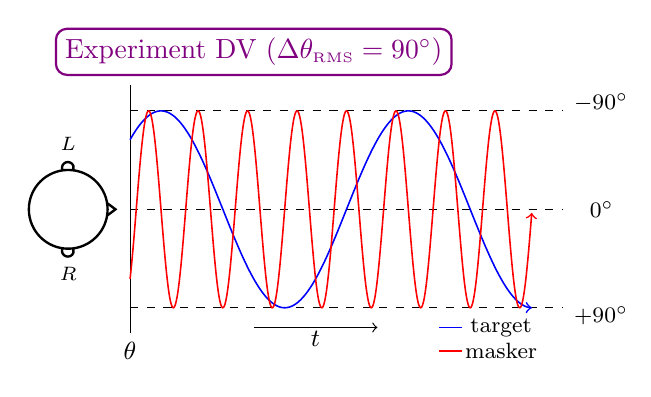
\begin{tikzpicture}
  % Title
  \node[thick, draw=violet, text=violet, rounded corners, opacity=1] at (3*pi/4, 2) {Experiment DV ($\Delta \theta_{\textrm{\tiny RMS}} = 90^{\circ}$)};
  
  % Legend
  \draw[line width=0.2mm, blue] (3*pi/2, -1.5) -- (3*pi/2 + 3*pi/32, -1.5);
  \node at (3*pi/2 + 8*pi/32, -1.5) {\footnotesize target};
  \draw[line width=0.2mm,  red] (3*pi/2, -1.8) -- (3*pi/2 + 3*pi/32, -1.8);
  \node at (3*pi/2 + 8*pi/32, -1.8) {\footnotesize masker};
  
  % y axis
  \draw[line width=0.125mm, black] (pi/4, -1.575) -- (pi/4, 1.575);
  \node at (pi/4, -1.8) {\small $\theta$};
  
  % Dashed degree guide lines
  \draw[line width=0.125mm, black, dashed] (pi/4,  1.25) -- (2*pi,  1.25);
  \draw[line width=0.125mm, black, dashed] (pi/4,  0.)   -- (2*pi,  0.  );
  \draw[line width=0.125mm, black, dashed] (pi/4, -1.25) -- (2*pi, -1.25);
  
  % Degree guides
  \node[align=right, text width=0.5cm] at (2*pi + pi/8,  1.35)
    {\footnotesize $-90^{\circ}$};
  \node[align=right, text width=0.5cm] at (2*pi + pi/8,  0.)
    {\footnotesize $0^{\circ}$};
  \node[align=right, text width=0.5cm] at (2*pi + pi/8, -1.35)
    {\footnotesize $+90^{\circ}$};
  
  % Arrow of time
  \draw[help lines, ->, line width=0.15mm, black] (3*pi/4, -1.5) -- (5*pi/4, -1.5);
  \node at (pi, -1.65) {\small $t$};
  
  % Sinusoids
  \draw[help lines, ->, line width=0.2mm, blue, domain=pi/4:2*pi - pi/8, samples=1000]
        plot(\x, {1.25*sin(( 2*\x - pi/4) r)});
  \draw[help lines, ->, line width=0.2mm,  red, domain=pi/4:2*pi - pi/8, samples=1000]
        plot(\x, {1.25*sin((10*\x - 3*pi/4) r)});
   
  % Head
  \node at (0, 0.825) {\scriptsize $L$};
  \draw[line width=0.3mm] (0, 0) circle (0.5cm); % head
  \draw[line width=0.3mm] (0 - 0.075,  0.5) arc ( 200:-20:0.075); % R ear
  \draw[line width=0.3mm]
         (0 + 0.5,  0.075) --
         (0 + 0.6,  0.   ) --
         (0 + 0.5, -0.075); % nose
  \draw[line width=0.3mm] (0 - 0.075, -0.5) arc (-200: 20:0.075); % L ear
  \node at (0, -0.825) {\scriptsize $R$};
\end{tikzpicture}



%%% Expt DV stim conditions
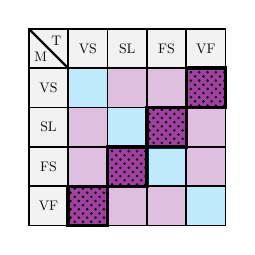
\begin{tikzpicture}[scale=0.5, every node/.style={transform shape}]
  % Target/Masker
  \node at (0.7, 4.7) {T};
  \node at (0.3, 4.3) {M};
  \draw[thick] (0, 5) -- (1, 4);
  
  % Row labels
  \node at (1.5, 4.5) {VS};
  \node at (2.5, 4.5) {SL};
  \node at (3.5, 4.5) {FS};
  \node at (4.5, 4.5) {VF};
  % Column labels
  \node at (0.5, 3.5) {VS};
  \node at (0.5, 2.5) {SL};
  \node at (0.5, 1.5) {FS};
  \node at (0.5, 0.5) {VF};
  
  % Row 1 (top)
  \draw[semithick, draw=black, fill=gray, fill opacity=0.1]
     (0, 4) -- (0, 5) -- (1, 5) -- (1, 4) -- cycle;
  \draw[semithick, draw=black, fill=gray, fill opacity=0.1]
     (1, 4) -- (1, 5) -- (2, 5) -- (2, 4) -- cycle;
  \draw[semithick, draw=black, fill=gray, fill opacity=0.1]
     (2, 4) -- (2, 5) -- (3, 5) -- (3, 4) -- cycle;
  \draw[semithick, draw=black, fill=gray, fill opacity=0.1]
     (3, 4) -- (3, 5) -- (4, 5) -- (4, 4) -- cycle;
  \draw[semithick, draw=black, fill=gray, fill opacity=0.1]
     (4, 4) -- (4, 5) -- (5, 5) -- (5, 4) -- cycle;
  % Row 2
  \draw[semithick, draw=black, fill=gray, fill opacity=0.1]
     (0, 3) -- (0, 4) -- (1, 4) -- (1, 3) -- cycle;
  \draw[semithick, draw=black, fill=cyan, fill opacity=0.25]
     (1, 3) -- (1, 4) -- (2, 4) -- (2, 3) -- cycle;
  \draw[semithick, draw=black, fill=violet, fill opacity=0.25]
     (2, 3) -- (2, 4) -- (3, 4) -- (3, 3) -- cycle;
  \draw[semithick, draw=black, fill=violet, fill opacity=0.25]
     (3, 3) -- (3, 4) -- (4, 4) -- (4, 3) -- cycle;
  \draw[very thick, draw=black, fill=violet, fill opacity=0.75]
     (4, 3) -- (4, 4) -- (5, 4) -- (5, 3) -- cycle;
  \draw[semithick, draw=black, pattern=crosshatch dots]
     (4, 3) -- (4, 4) -- (5, 4) -- (5, 3) -- cycle;
  % Row 3
  \draw[semithick, draw=black, fill=gray, fill opacity=0.1]
     (0, 2) -- (0, 3) -- (1, 3) -- (1, 2) -- cycle;
  \draw[semithick, draw=black, fill=violet, fill opacity=0.25]
     (1, 2) -- (1, 3) -- (2, 3) -- (2, 2) -- cycle;
  \draw[semithick, draw=black, fill=cyan, fill opacity=0.25]
     (2, 2) -- (2, 3) -- (3, 3) -- (3, 2) -- cycle;
  \draw[very thick, draw=black, fill=violet, fill opacity=0.75]
     (3, 2) -- (3, 3) -- (4, 3) -- (4, 2) -- cycle;
  \draw[semithick, draw=black, pattern=crosshatch dots]
     (3, 2) -- (3, 3) -- (4, 3) -- (4, 2) -- cycle;
  \draw[semithick, draw=black, fill=violet, fill opacity=0.25]
     (4, 2) -- (4, 3) -- (5, 3) -- (5, 2) -- cycle;
  % Row 4
  \draw[semithick, draw=black, fill=gray, fill opacity=0.1]
     (0, 1) -- (0, 2) -- (1, 2) -- (1, 1) -- cycle;
  \draw[semithick, draw=black, fill=violet, fill opacity=0.25]
     (1, 1) -- (1, 2) -- (2, 2) -- (2, 1) -- cycle;
  \draw[very thick, draw=black, fill=violet, fill opacity=0.75]
     (2, 1) -- (2, 2) -- (3, 2) -- (3, 1) -- cycle;
  \draw[semithick, draw=black, pattern=crosshatch dots]
     (2, 1) -- (2, 2) -- (3, 2) -- (3, 1) -- cycle;
  \draw[semithick, draw=black, fill=cyan, fill opacity=0.25]
     (3, 1) -- (3, 2) -- (4, 2) -- (4, 1) -- cycle;
  \draw[semithick, draw=black, fill=violet, fill opacity=0.25]
     (4, 1) -- (4, 2) -- (5, 2) -- (5, 1) -- cycle;
  % Row 5 (bottom)
  \draw[semithick, draw=black, fill=gray, fill opacity=0.1]
     (0, 0) -- (0, 1) -- (1, 1) -- (1, 0) -- cycle;
  \draw[very thick, draw=black, fill=violet, fill opacity=0.75]
     (1, 0) -- (1, 1) -- (2, 1) -- (2, 0) -- cycle;
  \draw[semithick, draw=black, pattern=crosshatch dots]
     (1, 0) -- (1, 1) -- (2, 1) -- (2, 0) -- cycle;
  \draw[semithick, draw=black, fill=violet, fill opacity=0.25]
     (2, 0) -- (2, 1) -- (3, 1) -- (3, 0) -- cycle;
  \draw[semithick, draw=black, fill=violet, fill opacity=0.25]
     (3, 0) -- (3, 1) -- (4, 1) -- (4, 0) -- cycle;
  \draw[semithick, draw=black, fill=cyan, fill opacity=0.25]
     (4, 0) -- (4, 1) -- (5, 1) -- (5, 0) -- cycle;
\end{tikzpicture}

\end{tabular}

%%%%%%%%%%%%%%%%%%%%%%%%%%%%%%%%%%%%%%%%%%%%%%%%%%
%%%%%%%%%%%%%%%%%%%%%%%%%%%%%%%%%%%%%%%%%%%%%%%%%%
\end{document}